\textbf{Problem definition}:
Apply Harmonic Balance to obtain the response of a Duffing oscillator where the governing equation is defined as
%
\begin{equation}\label{eq:Q2_GE}
	\ddot{x} + 
	\left( 0.01 + \frac{\alpha}{100} \right) \dot{x} +
	x + \frac{\alpha}{10} x^3 = \sin 3t
	\qquad
	\text{where }
	\alpha = 12
\end{equation}
%

\noindent\hrulefill

% -------------------------------------------------------------------
\textbf{Solution approach:}
To solve Equation \eqref{eq:Q2_GE} using the Harmonic Balance (HB) method, we first define the residual function as
%
\begin{equation}\label{eq:Q2_residualFunction}
	\mathcal{R} =
	\ddot{x} + 
	\left( 0.01 + \frac{12}{100} \right) \dot{x} +
	x + \frac{12}{10} x^3 - \sin 3t
\end{equation}
%
we then assume a solution $\bar{x}$. If $\bar{x}$ is indeed the solution of Equation \eqref{eq:Q2_GE}, when substituting it in the residual equation of \eqref{eq:Q2_residualFunction} we should get zero. However, since it is an assumed solution, the residual won't be zero. By updating $\bar{x}$ is an optimization loop to minimize $\mathcal{R}^2$, we can get the solution of Equation \eqref{eq:Q2_GE}. In this process, it is required to calculate $\ddot{x}$ and $\dot{x}$ for $\mathcal{R}$. This is done in frequency domain.

The variable $x$ in the time domain can be approximated as follows in the frequency domain.
%
\begin{equation}\label{eq:Q2_displacement}
	x(t) = 
	\sum_{k=-\infty}^{\infty}
	X_k \cdot e^{i \omega_0 k t} \quad , \quad \omega_0 = \frac{2\pi}{T}
\end{equation}
%
The time derivatives are calculated by differentiating above equation with respect to time.
%
\begin{subequations}
\begin{equation}\label{eq:Q2_velocity}
	\dot{x}(t) = \sum_{k=-\infty}^{\infty} i \omega_k X_k \cdot e^{i \omega_k t}
\end{equation}
\begin{equation}\label{eq:Q2_acceleration}
	\ddot{x}(t) = \sum_{k=-\infty}^{\infty} -\omega_k^2 X_k \cdot e^{i \omega_k t}
\end{equation}
\end{subequations}
%
By substituting Equations \eqref{eq:Q2_displacement}, \eqref{eq:Q2_velocity}, and \eqref{eq:Q2_acceleration} into Equation \eqref{eq:Q2_residualFunction}, we can minimize the residual based on a guessed displacement. The flow chart for this is shown in Figure \ref{fig:Q2_flowchart}.
%
\begin{figure}[h]
	\centering
	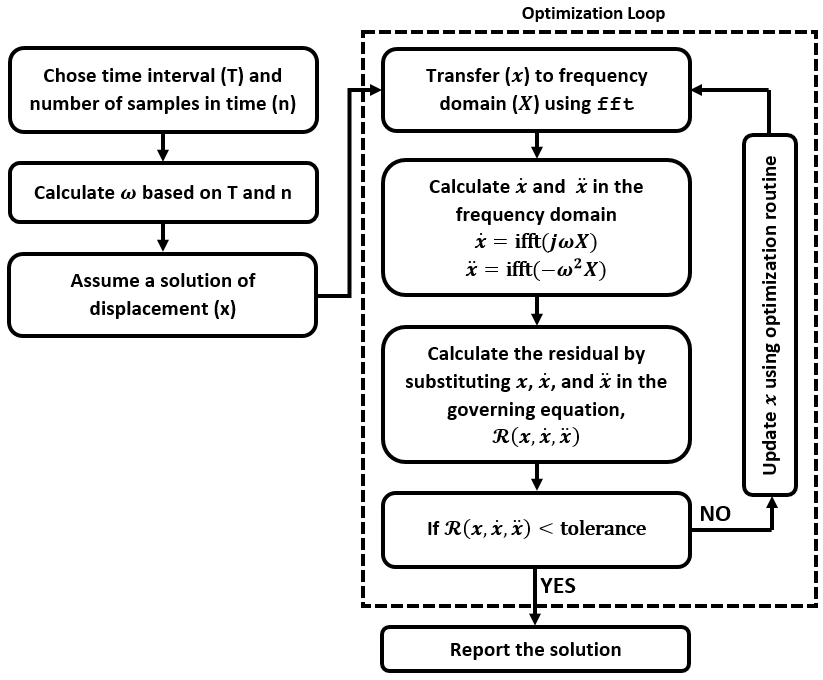
\includegraphics[width=10.0cm]{figure/Q2/minimize_residual.png}
	\caption{Flowchart for numerical approach.}
	\label{fig:Q2_flowchart}
\end{figure}
%

To transfer the time domain data for frequency domain we use \texttt{numpy.fft.fft} function and for converting the frequency domain data back to time domain we used \texttt{numpy.fft.ifft}. We sampled the frequency domain using $19$ points. The initial guess for displacement is selected as a vector of ones, \texttt{numpy.ones}. It should be noted that this is a vector of displacement in time. The minimization of residual is done using python \texttt{scipy.optimize.minimize} function using \texttt{SLSQP} method. The convergence plot for the residual function is shown in Figure \ref{fig:Q2_residualConvergence}. The horizontal lines in this graph represent the steps used to calculate the finite difference derivatives of the residual with respect to each of design variables (number of $x$ points in time). As can be seen here, the residual function is minimized at the end of optimization stage.
%
\begin{figure}[h]
	\centering
	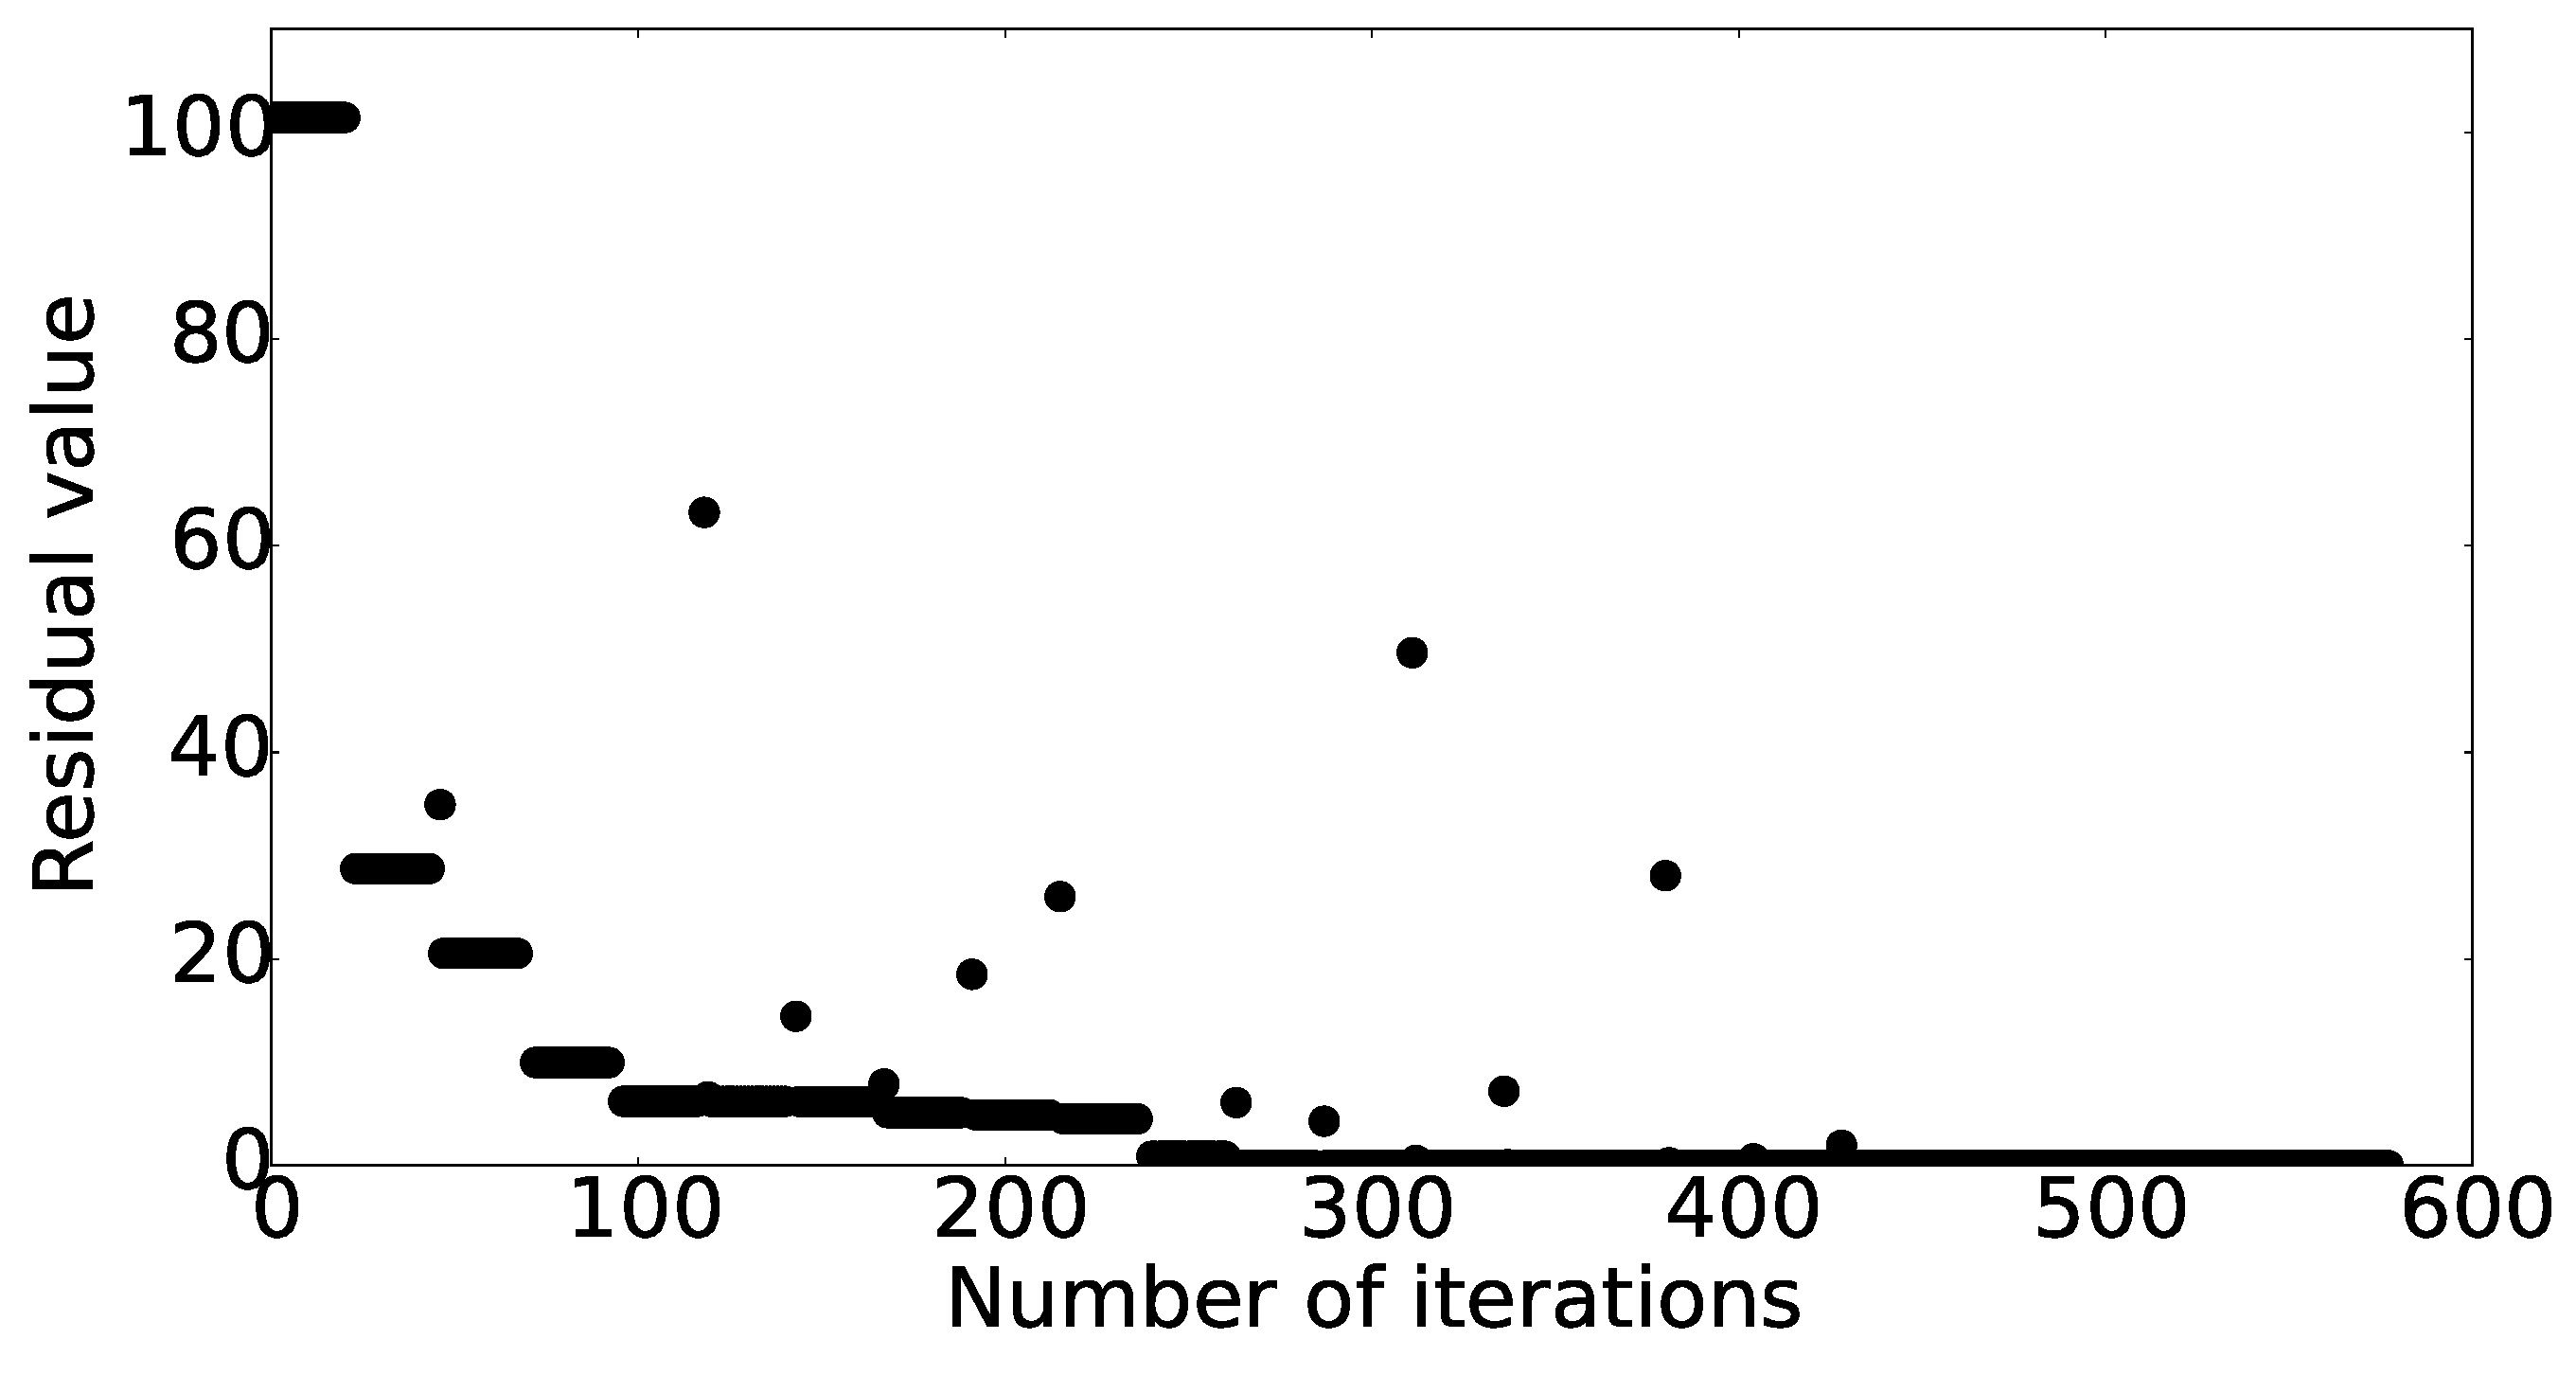
\includegraphics[width=10.0cm]{figure/Q2/convergence_study.eps}
	\caption{Convergence of residual.}
	\label{fig:Q2_residualConvergence}
\end{figure}
%

To verify the result of HB method, we used numerical integration to calculate the solution of Equation \eqref{eq:Q2_GE}. It should be noted that HB is capable of capturing the steady-state response of the system. Therefore, it is required to let the transient response of the time integration to die of before comparing the results. This comparison is shown in Figure \ref{fig:Q2_verification}.
%
\begin{figure}[h]
	\centering
	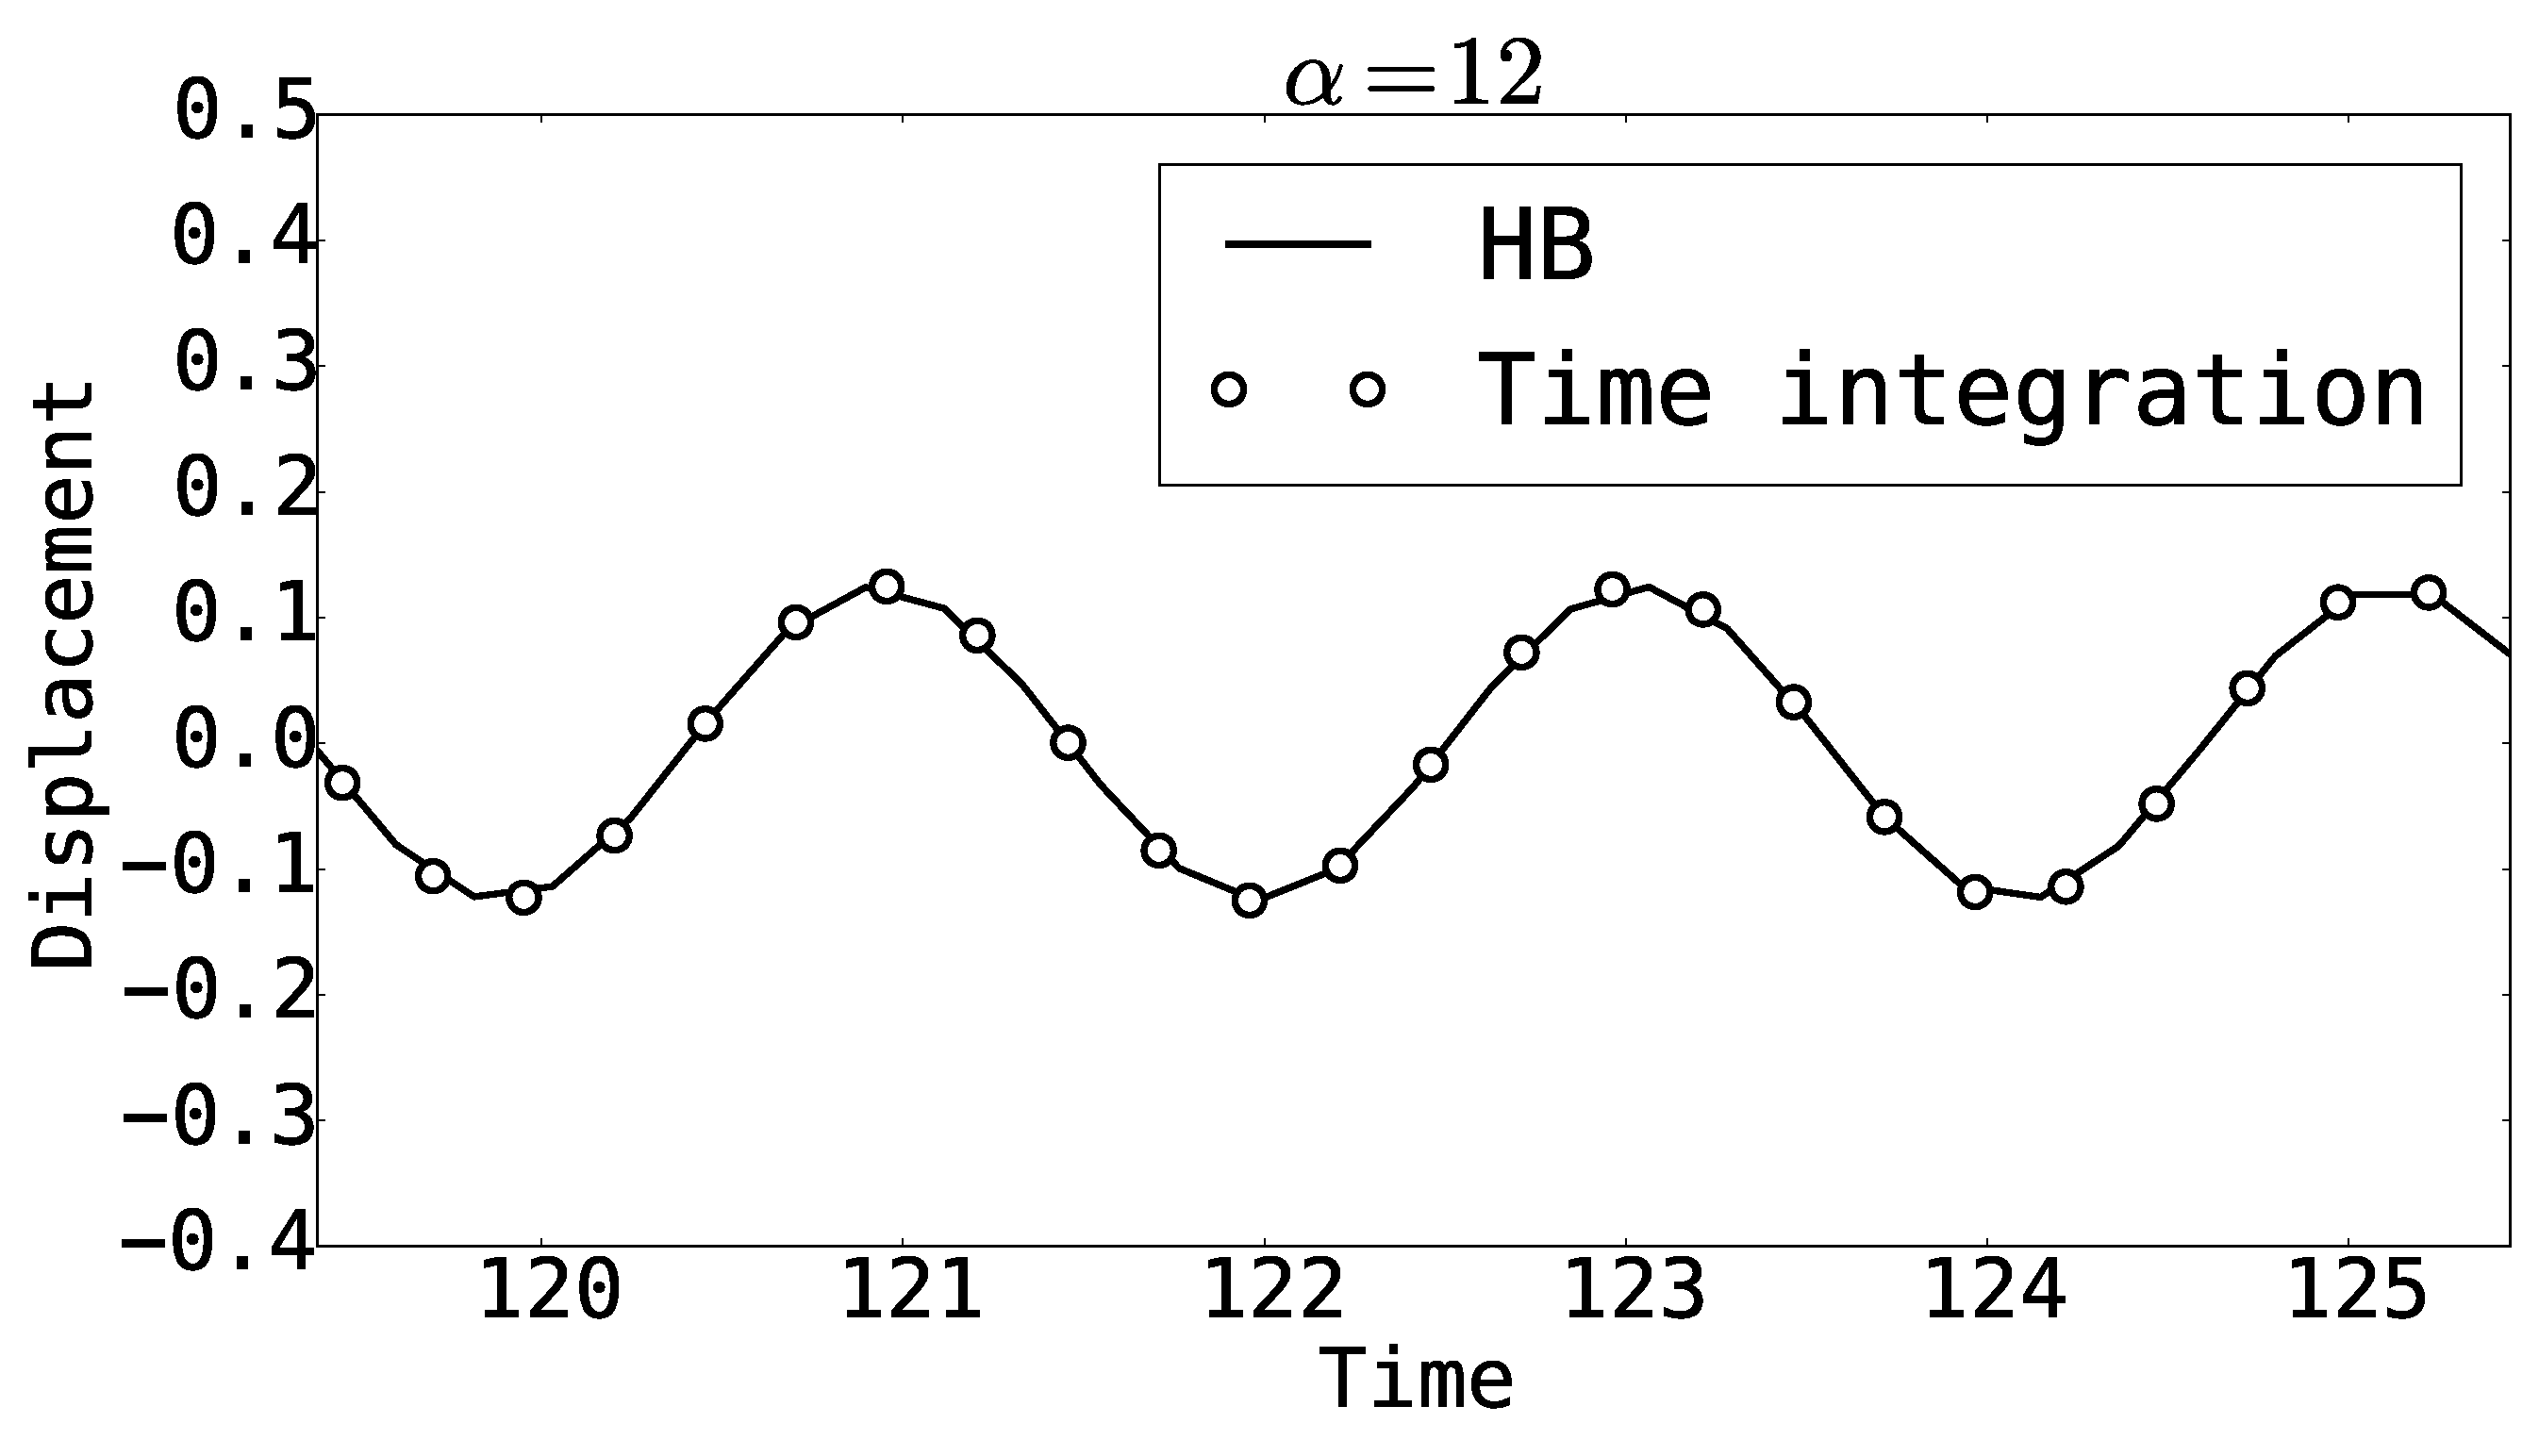
\includegraphics[width=10.00cm]{figure/Q2/HB_verification.eps}
	\caption{Comparison between HB and time integration results.}
	\label{fig:Q2_verification}
\end{figure}
%

The numerical results of HB can be written in terms of trigonometric functions. This is done using fast Fourier transforms as well. The results of \texttt{numpy.fft.fft} is a vector in frequency domain where its values are the coefficients of trigonometric functions with appropriate frequencies. In particular the real portion of the \texttt{fft} results is the cosine transform and the imaginary portion is the sine transform of the vector in time domain. The frequency corresponding to the \texttt{fft} vector of length $N=9$ can be written as:
%
\begin{equation}\label{eq:Q2_frequencyData}
	\omega_k = \frac{2 \pi}{T}
	\begin{bmatrix}
	0 & 1 & 2 & 3 & 4 & -4 & -3 & -2 & -1
	\end{bmatrix}
\end{equation}
%
Using Equation \eqref{eq:Q2_frequencyData} and the real and imaginary portion of \texttt{numpy.fft.fft} vector, the time domain results can be reconstructed upto $n$ harmonics where $n \leq k$. $k$ is the number of harmonics used in calculating the response using HB method. Using this approach, the result of approximated using $3$ harmonics is as follows
%
\begin{align*}
	x(t) = 
	&- 1.6074 \times 10^{-4} \\
	&+ 1.3664 \times 10^{-5} \cos t - 1.4597 \times 10^{-5} \sin t \\
	&+ 4.6340 \times 10^{-5} \cos 2t + 3.6900 \times 10^{-5} \sin 2t \\
	&+ 6.0986 \times 10^{-3} \cos 3t + 1.2491 \times 10^{-1} \sin 3t
\end{align*}
%
Because most of the coefficients are small, above is approximated as
%
\begin{equation}\label{eq:Q2_solution}
	x(t) = 0.12491 \sin 3t
\end{equation}
%
The comparison between approximating the solution of Equation \eqref{eq:Q2_GE} by \eqref{eq:Q2_solution}, HB with $19$ terms and numerical integration is shown in Figure \ref{fig:Q2_resultVerification}. As can be seen here, the results match very well.
%
\begin{figure}[h]
	\centering
	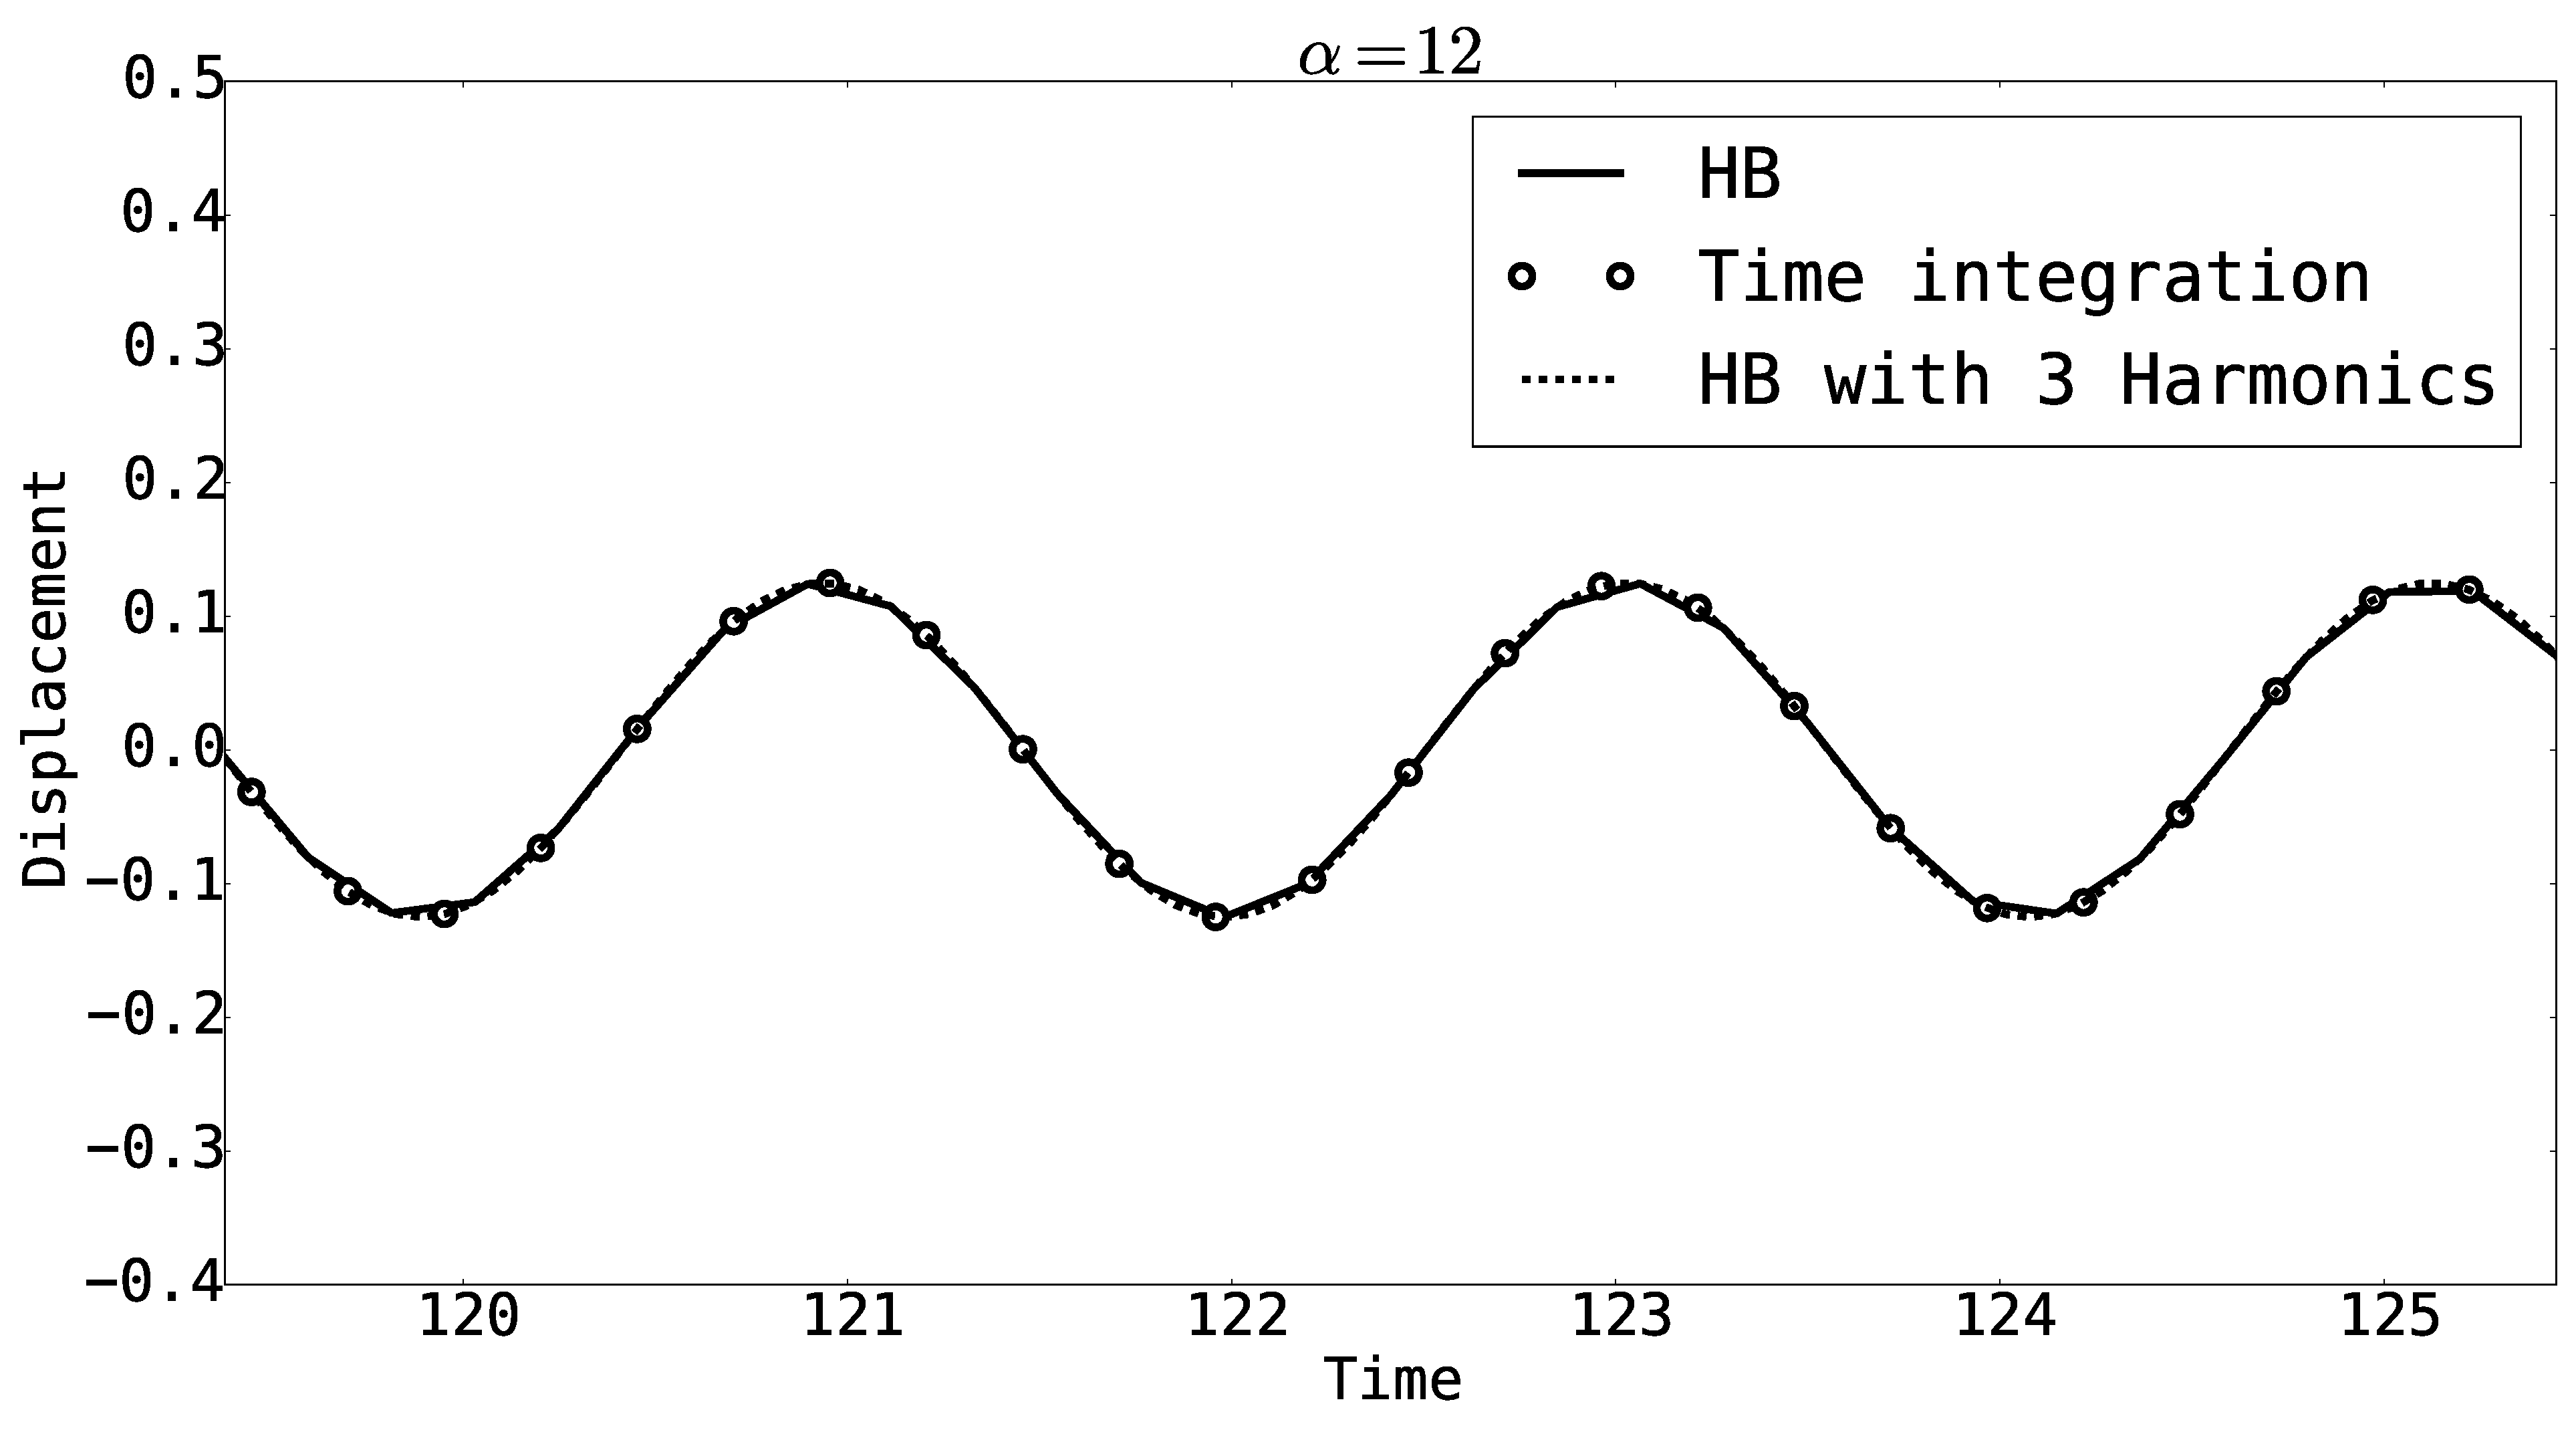
\includegraphics[width=10.00cm]{figure/Q2/HB_resultVerification.eps}
	\caption{Comparison between HB and time integration results.}
	\label{fig:Q2_resultVerification}
\end{figure}
%
The \texttt{python} code used for this problem is included in the following pages.